%!TEX root = ../main.tex
\section{SLOC Approach Overview}
\label{sec:Approach}

\subsection{Main Objectives} 
To address the aforementioned challenges and 
achieve our vision of SLO-native paradigm for the next generation cloud
platforms, our SLOC framework sets the following main objectives.
\todo{Map the challenges to objectives}

\begin{itemize}
	\item \todo{We want to enable the users to specify the SLOs in terms which are aligned with their business requirements. The customers are interested in their app performance (business requirements) and don't care 
	about resources per se. For example, the costs can be the main decision driving factor.} 
	\item \todo {We are intending to use elasticity mechanisms to support and enforce/guarantee SLOs}
	\item In order to achieve formally verifiable requirements of both the Cloud 
elasticity and the application (e.g., SLOs), our framework intends to develop 
{\em SLO-native elasticity models}. This will facilitate formal reasoning on and 
verification of multidimensional elasticity and SLOs, from the early stages 
of design. 
\item In order to enable the shift from low-level, resource-centered SLOs 
and elastic requirements specification to {\em intent-focused, 
multidimensional elasticity models and performance-centered SLOs}, 
our framework will provide novel 
coordination, control, and orchestration approaches that enable Cloud systems 
to adapt dynamically to varying load patterns in a dependable manner.
\end{itemize}

\subsection{Main Concepts and Architecture Overview}
The core idea behind SLOC framework is to enable SLO-native management of 
elastic Cloud resources. 
\todo{In a nutshell,} our {\em SLO-native approach} introduces a 
paradigm shift from general, business logic agnostic, low-level SLAs to  
{\em intent-based, SLO-first, performance-driven and orchestration-aware} 
elasticity models.

\begin{enumerate}
	\item Intent-based means that we are declaring what the execution environment
	of a workload should look like i.e., the infrastructure/resource desired state for 
	the given point in time considering the elasticity requirements, constraints and SLAs.
	\item SLO-first means that all the SLOs and QoS along multiple elasticity 
	dimensions are inherently aligned with application model and business 
	requirements/KPIs as opposed to external, business logic agnostic configurations.
	\item Performance driven
	\item Orchestration-aware implies that the application deployment bundles
	such as microservices or service mashes are aware of automated deployment, 
	scaling, scheduling and management.
\end{enumerate}
%
\begin{figure}[t]  
\centering
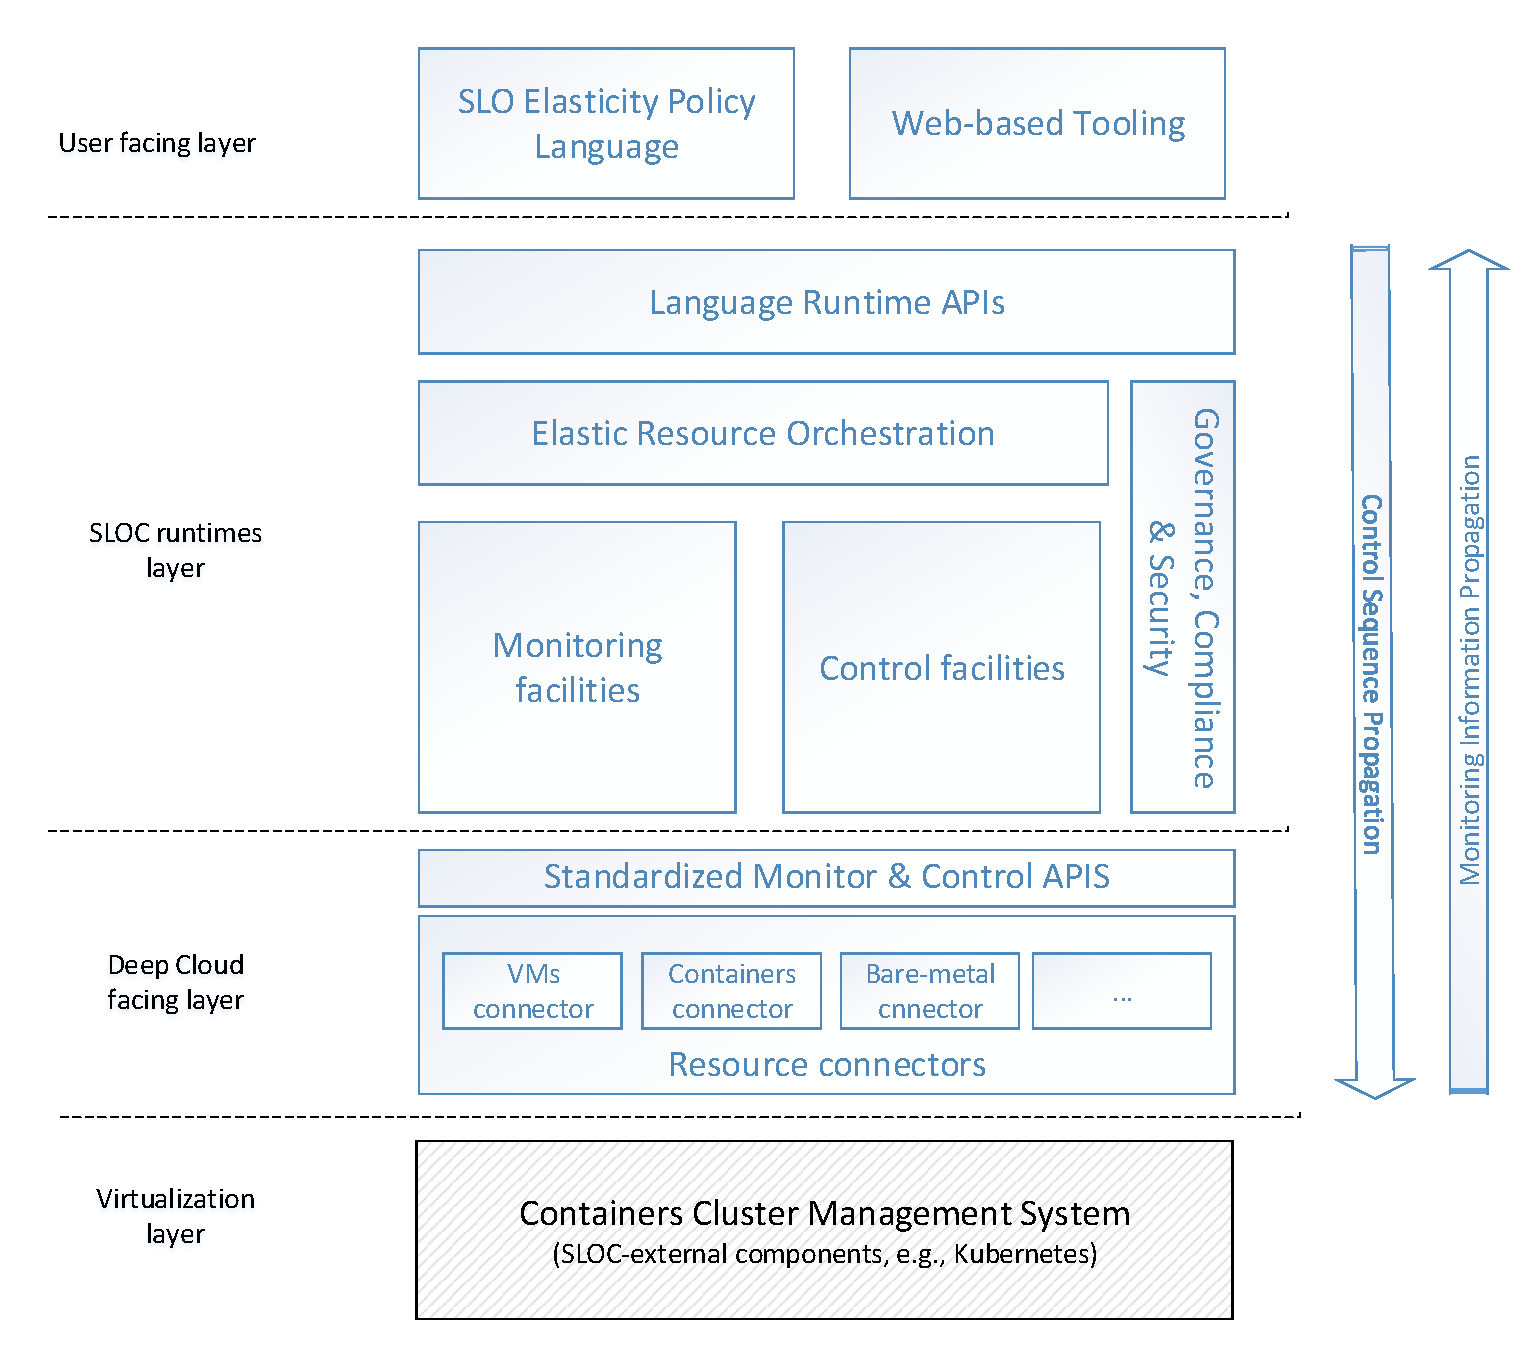
\includegraphics[width=0.8\columnwidth]{figures/sloc_architecture}
\caption{SLOC Architecture Overview.}
\label{fig:architecture}
\end{figure}% 
%
Subsequently, we outline the architecture of our SLOC framework
and give an overview of its main components.
Figure~\ref{fig:architecture} shows a high-level view of the 
framework architecture together with main control 
processes (top-down) and monitoring data delivery and analytics
process (bottom-up).
%
On a high-level we identify three main layers of SLOC framework:
\begin{inparaenum}[i)]
  \item User-facing layer,
  \item SLOC runtimes layer, and
  \item Deep Cloud facing layer.
\end{inparaenum}

The User-facing layer exposes main abstractions, mechanisms
and runtime services of the SLOC framework to the end users,
enabling them to define SLO elastic policies, visualize their
infrastructure and its current status, as determined by SLOC's
observability mechanisms. We discuss SLOC's SLO Elastic 
Policy Language in detail in Section~\ref{sec:mechanisms}.

The SLOC runtimes layer is the ``brains'' of our framework.
Generally, it is responsible for implementing main models, algorithms and
mechanisms, which are required to interpret user-defined SLOs,
translates such SLOs and QoS requirements in cloud-specific
resource \todo{configurations} and enforce such SLOs during runtime.
The most important components at this layer include:
\begin{inparaenum}[i)]
  \item Elastic Resource Orchestration,
  \item Observability facilities, 
  \item Control facilities, and
	\item Governance, Compliance \& Security Concerns.
\end{inparaenum}
%
The Elastic Resource Orchestration is responsible for interpreting and 
executing user-defined SLOs, elasticity requirements and 
configuration models.  
This layer acts as a ``gluing'' component bringing together SLO 
definitions, multi-dimensional elasticity models and framework's 
runtime mechanisms. For example, Elastic Resource 
Orchestration receives policy configuration directives, 
in terms of high-level objectives such as to optimize 
infrastructure for latency. It interprets these objectives 
and decides how to orchestrate the underlying resources, 
by invoking the underlying  runtime mechanisms as well as 
delegating specific decisions and/or responsibilities
to cluster management system controllers. 
%For example, it can utilize the Scheduling and 
%the Placement mechanisms to determine the most suitable 
%node for a service in order to reduce the network latency.
The details of Observability and Control facilities are
discussed in Section~\ref{sec:mechanisms}.

SLOC's third key layer is the Deep Cloud facing layer.
\todo{finish}

